\documentclass[conference]{IEEEtran}
\usepackage[pdftex]{graphicx}
\usepackage[cmex10]{amsmath}
\interdisplaylinepenalty=2500
\usepackage{array}
\usepackage{mdwmath}
\usepackage{mdwtab}
\usepackage{eqparbox}
\usepackage[font=footnotesize]{subfig}
\usepackage{fixltx2e}
\usepackage{url}
\hyphenation{}

% additional packages and utility commands

\usepackage{float}

\newcommand{\TODO}{\textbf{\color{red}TODO}}

% \usepackage{flushend}

% while preparing, linenumbers come in handy
\usepackage{lineno}
\setlength\linenumbersep{1mm}
\linenumbers

% until we settle on the final name ;-)
\usepackage{xspace}
\newcommand{\NAME}{id-foo\xspace}

% http://tex.stackexchange.com/questions/299/how-to-get-long-texttt-sections-to-break
\newcommand*\justify{%
  \fontdimen2\font=0.4em% interword space
  \fontdimen3\font=0.2em% interword stretch
  \fontdimen4\font=0.1em% interword shrink
  \fontdimen7\font=0.1em% extra space
  \hyphenchar\font=`\-% allowing hyphenation
}

% http://en.wikibooks.org/wiki/LaTeX/Customizing_LaTeX
\newcommand{\ttt}[1]{\texttt{\justify{#1}}}

\usepackage{algpseudocode}
% custom Let command
\newcommand*\Let[2]{\State #1 $\gets$ #2}
\renewcommand{\algorithmicforall}{\textbf{for each}}
\let\ForEach\ForAll

\usepackage{listings}

\usepackage{tikz}
\usetikzlibrary{positioning}
\usetikzlibrary{calc}
\usetikzlibrary{graphs}
\usetikzlibrary{trees}
\usetikzlibrary{arrows}

\usepackage{tikz-3dplot}

%!TEX root=paper.tex

% basics

\tikzset{
  box/.style            = { rectangle, minimum width=2cm, minimum height=1cm },
  border/.style         = { thick, draw=black },
  round/.style          = { rounded corners=3mm },
}

% system

\tikzset{
  artifact/.style       = { box, font=\ttfamily },
  support/.style        = { box, font=\itshape },
  user/.style           = { artifact, fill=black!15!white },
  dom/.style            = { support,  fill=black!30!white },
  platform/.style       = { support,  fill=black!55!white, text=white },
  native/.style         = { support,  fill=black!70!white, text=white },
  generated/.style      = { artifact, border, dashed },
  resource/.style       = { artifact, border },
  representation/.style = { support, border, round }
}

% UML

\tikzset{
  class/.style={
    box,
    border,
    text centered,
    text width=1.75cm
  },
  relation/.style       = { thick, draw=black, <-},
  subclass/.style       = { relation, >=open triangle 60 },
  aggregate/.style      = { relation, >=open diamond },
  composite/.style      = { relation, >=diamond },
  dependency/.style     = { relation, >=latex, -> }
}

\lstdefinelanguage{foo-lang}{
  emph={module,const,from,import,extend,with,after,do,function,@every,having,if,return},
  emphstyle={\textbf},
  morecomment=[l]{//},
  moredelim=[is][]{@@}{@@},       % temp solution to allow keywords without emph
  moredelim=[is][\emph]{!!}{!!}   % temp solution to hightlight #atoms
}


\usepackage[autostyle]{csquotes}

\usepackage{booktabs}
\usepackage{multirow}
\usepackage{stfloats}



\begin{document}

\title{
\NAME: A framework for \\
Efficient Intrusion Detection\\
in the Internet of Things
}

\author{\IEEEauthorblockN{Christophe Van Ginneken, Jef Maerien,
Christophe Huygens, Wouter Joosen, Danny Hughes}%
\IEEEauthorblockA{iMinds-DistriNet, KU Leuven\\
3001 Leuven, Belgium\\
\{firstname.lastname\}@cs.kuleuven.be}}

\maketitle

\begin{abstract}

When intrusion prevention fails, intrusion detection serves as a second layer
of defense. It looks for patterns and anomalies that can indicate malicious
behavior. However, supporting an adequate set of intrusion detection algorithms
imposes significant overhead on resource-constrained devices such as those in
the Internet of Things. Manual fusion of the algorithms reduces resource
consumption by optimizing resource sharing, yet, proves to be time-consuming,
repetitive and error-prone. To address this problem we propose \NAME, a
framework for the development of efficient intrusion detection systems. It
consists of a domain specific language and a code generator. The language
allows formally describing the intent of intrusion detection algorithms and
supports the generator in organizing the source code. A side-by-side comparison
shows that \NAME-generated code reduces message passing overhead, execution
time and memory footprint in comparison to sequential calls to individual
implementations of the algorithms.

\end{abstract}

\section{Introduction}

% context

% wired networks: fw and central ids

In wired networks, firewalls focus on the outer perimeter of the network,
filtering unwanted packets and protecting the entire internal network. But
attacks on flaws in services can pass unnoticed. This is where intrusion
detection (ID) comes into play: an intrusion detection system (IDS) monitors
all traffic that passes through the firewall, looking for patterns of malicious
activity, and optionally, after detecting such pattern, alerts the firewall,
allowing it to take corrective actions \cite{denning1987intrusion}.

% IoT + threat

The internet of things (IoT) holds great potential to positively influence our
daily work and life through domotics, assisted living, e-health and enhanced
learning \cite{atzori2010internet}. But with this potential the IoT also
presents a significant threat: by opening our smart homes and personal data to
all of these interconnected devices, we also open them to everyone who is able
to break the virtual locks that protect them (i.e.\ passwords \& encryption
keys). Implementation of security measures by itself is hindered by the fact
that IoT devices typically have limited batteries, processing power and memory.

% local ids -> localize -> limited resources

In wireless networks of resource-constrained devices, which make up a
significant part of the IoT, it is not possible for a single point in the
network to oversee all traffic \cite{mishra2004intrusion}. Every device has to
implement its own lines of defense. However making the IDS a local service on
each device requires local resources, which are a scarce commodity for IoT
devices.

Attackers have access to a large set of possible attack vectors
\cite{aschenbruck2012security}, ranging from the physical layer, through the
access and routing layers, up to the application layer. Each layer presents
different opportunities to manipulate data, eavesdrop or perform a form of
denial of service. For each of these attacks an algorithm needs to look for
patterns or anomalies. An IDS for IoT devices therefore requires a large number
of algorithms for an adequate coverage.

% gap analysis

Current developments in ID on resource-constrained devices focus on programming
frameworks that structure the implementation of algorithms \cite{valero2012di}
and offer the required basic functional components to implement them
\cite{krontiris2008lidea}. A key shortcoming of prior ID frameworks, is that
they don't offer a way to optimize the usage of resources. A solution that
supports the integration of multiple algorithms on IoT devices needs to avoid
accumulating their impact on the available resources. A second omission is
support for systematic reuse to create different configurations. Addressing
this in a transparent and automated way offers the potential to significantly
reduce the effort of developing an IDS.

% scientific contribution

% 1. classification of ID and design pattern for ID algorithms

The first contribution of this paper consists of the formulation of a design
pattern for ID algorithms, based on properties identified from a classification.

% 2. framework: language + code generator

The second contribution is a framework called \NAME. It enables the formal
description of ID algorithms on a functional level and provides a code
generator producing source code for a given platform and configuration. This
way, \NAME addresses the heterogeneous nature of both IoT and ID algorithms.

% 3. FCF to optimise

The third contribution introduces functional code fusion (FCF) as a source code
generation paradigm to address hard to combine ID algorithms. FCF identifies
common data and functions, and organizes code to eliminate redundant
iterations, tests and computations. Results show reduced usage of the wireless
radio, execution time and memory usage.

% structure

The remainder of this paper proceeds as follows: section \ref{problems}
describes the inherent problems with the combination of ID algorithms. Section
\ref{classification} analyses and classifies ID algorithms. Section
\ref{pattern} looks for patterns in the implementation of these classes.
Section \ref{design} describes the design we applied to construct \NAME, its
domain specific language (DSL) and code generator. Section \ref{evaluation}
discusses and evaluates an implementation. Section \ref{related} explores
related work in the field of DSLs and code generation. Finally, section
\ref{conclusion} summarizes our findings, draws conclusions and identifies
topics for future work.

\section{Inherent Problems}
\label{problems}

The combination of multiple ID algorithms tends to result in suboptimal code.
Besides these code-level problems, operational problems also hinder the
implementation of an IDS for IoT devices.

Two issues arise from the way ID algorithms are implemented and deal with loop
constructs and common data. A third issue is the use of the network.

\begin{LaTeXdescription}

  \item[Loops] by themselves are not a problem, but different loops, that
  perform the same operations in sequence, can incur overhead. An example is
  the handling of messages: each algorithm parses each observed message on the
  network, processing the same byte stream, performing comparable operations to
  find similar patterns.

  \item[Common data] cross-cuts the different algorithms, that have to store
  information about devices within its own scope. This results in a lot of
  duplicated information in memory.

  \item[The network] allows algorithms to operate on a distributed scale. But
  scattered calls to the a message sending function cause multiple accesses to
  the wireless radio, keeping it active and energy consuming more than strictly
  needed.

\end{LaTeXdescription}

Two operational aspects are orthogonal to these problems and amplify them:

\begin{LaTeXdescription}
  
  \item[Reimplementing] the algorithms manually to eliminate these issues is
  not a one-time cost. A release of a new version of an algorithm, or simply a
  reselection of algorithms, due to a changing risk analysis, can trigger it.
  Also, changing, or simply implementing the algorithms from scratch, holds the
  risk of making mistakes.

  \item[The heterogeneity of IoT devices] results in different software stacks,
  each with for example their own network API\@. This partially explains why
  there are few implementations readily available to developers: there is no
  single platform to target for researchers.

\end{LaTeXdescription}

\section{A Classification of ID Algorithms}
\label{classification}

Two aspects currently missing from ID frameworks are optimization of resources
and support for systematic reuse. This section uses a classification to define
the scope of \NAME, detailing which types of algorithms are good candidates for
the proposed approach.

Research into ID in wireless networks typically focuses on two major topics:
the devices as single entities and the network as a group of such devices. Both
are important: a group cannot make a decision without members that detect
malicious behavior and a group-based decision is often needed because devices
in the network can miss certain events that could reveal intrusions. In a
wireless network, where not all participants are within each others' radio
range, wireless devices typically only have a partial view on the entire
network. This prohibits them from observing potentially crucial events in
distant parts of the network. The fact that resource-constrained devices
typically apply duty cycling to lower their energy consumption, further
increases this problem, introducing periods of time where they cannot observe
local events.

This leads to two complementary classes of ID activities: local intrusion
detection and cooperative decision making.

\subsection{Local Intrusion Detection}
\label{detection}

There are different ways to construct a taxonomy for intrusion detection, but
common themes do appear. According to \cite{mishra2004intrusion} and
\cite{ioannis2007towards} there are three major categories: 1) anomaly
detection, 2) signature or misuse detection, and 3) specification-based
detection. In \cite{alrajeh2013intrusion} the authors agree with this typology
and add the notion of hybrid intrusion detection systems and cross layer
intrusion detection systems as recent advances in research. Although these
additional categories seem promising, the authors admit that the impact on
resource-constrained devices will be too much. We therefore focus on the three
categories agreed upon by most sources.

\begin{LaTeXdescription}
  
  \item[Anomaly detection] considers a baseline profile and evaluates all
  activity according to this profile. It tries to flag aberrant behavior as a
  possible intrusion. The baseline profile can evolve over time, especially in
  wireless and mobile environments. Single events should therefore not result
  in absolute decisions.
  
  \item[Signature or misuse detection] starts with known patterns of attacks.
  It tries to find evidence for intrusions in the actions of and communication
  with a device. Because attacks often use valid ways to communicate with
  services on the devices, this approach can produce false positives.
  
  \item[Specification-based detection] uses constraints that describe the
  correct behavior of the system. Although this approach can detect previously
  unknown attacks, it can sometimes not detect specific attacks that anomaly or
  misuse detection can.
  
\end{LaTeXdescription}

\subsection{Cooperative Decision Making}
\label{coorperative}

These taxonomies focus on the act of detecting intrusions themselves. In a
distributed environment, communication between participants may be even more
important.

Because not all devices are always actively participating in the network, they
can miss events that would otherwise lead them to detect intrusions. It is
hardly impossible for a single device to detect a complex attack by itself.
Therefore a second important class of ID algorithms consists of cooperative
algorithms that combine information from single identities into a group-based
decision about alleged intrusions. We identify two ways to construct
cooperative decision making and focus on the way participants exchange
information: broadcast and interactive communication.

\begin{LaTeXdescription}

  \item[Broadcast communication] can allow implementing a distributed,
  cooperative algorithm locally: devices can exchange information about the
  reputation of other devices, solely using one-way broadcast messages.
  Combining this information allows them to decide about their trust in a given
  device, based on more than their own, often partial, observations. The
  reputation-based detection algorithm introduced in
  \cite{ganeriwal2008reputation} illustrates this. It uses the same principle
  of a watchdog found in \cite{mishra2004intrusion}.

  \item[Interactive communication] allows algorithms to exchange information to
  reach a consensus. In \cite{krontiris2009cooperative}, the authors first
  present a theoretical foundation to analyze cooperative algorithms. Given
  these foundations they continue to present an algorithm consisting of five
  phases, which essentially implement a voting system based on the Guy Fawkes
  protocol \cite{anderson1998new}, to identify an intruder. It enables the
  exchange of suspected intruder information and allows for distributed
  authentication of those \emph{votes}. Based on these authenticated votes, the
  participants can make a distributed decision about the jointly identified
  intruder.

\end{LaTeXdescription}

\subsection{Properties and Scope of \NAME}
\label{scope}

Figure \ref{fig:classification} visually summarizes the dual classification and
scope of \NAME.

\begin{figure}[ht]
  \centering
  \scalebox{.85}{
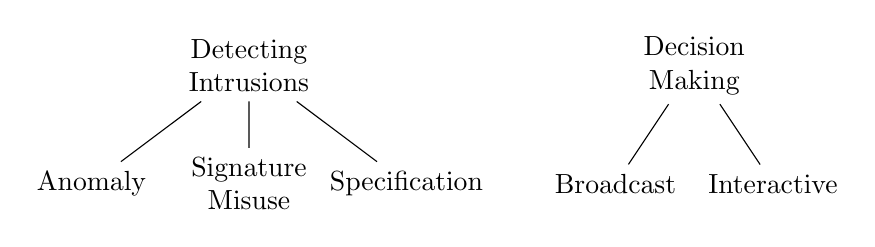
\begin{tikzpicture}[
  sibling distance=20mm,node distance=40mm
  ]
  \node (detection)             [align=center] {Detecting\\Intrusions}
    child {node (anomaly)       [align=center] {Anomaly}}
    child {node (signature)     [align=center] {Signature\\Misuse}}
    child {node (specification) [align=center] {Specification}};
  \node (decision)              [align=center,right=of detection] {Decision\\Making}
    child {node (broadcasting)  [align=center] {Broadcast}}
    child {node (interactive)   [align=center] {Interactive}};
\end{tikzpicture}
}
  \caption{Classification of ID Algorithms}
  \label{fig:classification}
\end{figure}

Algorithms that fit this classification are typically platform independent.
They look for patterns in network messages that can reveal intrusions and, in
doing so, all deal with the same information: other devices in the network. To
be able to formally describe ID algorithms and target the heterogeneous IoT,
\NAME requires ID algorithms to expose these properties.

A class of ID algorithms that does not have these properties is software
attestation \cite{seshadri2008sake}. It enables exchanging information about
the software that is running on a device and identifying devices with modified
content. These algorithms are highly platform dependent and have no data in
common with other algorithms, as they look for the effects of an intrusion, not
the intruder itself.

\section{A Design Pattern for ID Algorithms}
\label{pattern}

Based upon the classification presented in section \ref{classification}, we now
introduce a design pattern that identifies common functional aspects of ID
algorithms. It will allow us to define a strategy for optimizing the
combination of these algorithms. We extract two activities common to most
algorithms: the inspection of network traffic and the evaluation of thresholds.

Network traffic is the carrier along which malicious payloads reach a device
directly. Indirectly a device can also detect aberrant patterns of
communication by other devices, as a result of a successful attack.

Not all algorithms can decide if an attack is real or not, based on a single
event. Signature and misuse detection can in some cases, but anomaly detection
typically deals with some level of uncertainty. Also, in distributed setups it
is impossible to fully trust any neighboring device. In these situations one
has to rely on statistics and thresholds to decide when to drop trust in a
given device.

Updating such statistics and evaluating the corresponding thresholds should be
distinct operations. The example of a watchdog \cite{mishra2004intrusion}
illustrates this: a device monitors the actions of other devices and checks if
they correctly forward messages to distant nodes in the network. Missing
forwards can indicate a malicious intension to silently drop messages and
obstruct the normal operation of the network. There are valid reasons why a
device can miss the theoretical window in which one expects activity, i.e.\ the
wireless network being the most predominantly unreliable component. Directly
reacting upon a basic threshold can result in false positives. A way to
overcome this is to decouple the detection of problems and the decision what to
do about them.

This decoupling of detection and decision is the core of the design pattern for
ID algorithms. Listing \ref{alg:id-algo-pattern} presents the design pattern in
pseudo-code.

\begin{figure}[ht]
\captionof{lstlisting}{ID Algorithm Pattern\label{alg:id-algo-pattern}}
\begin{algorithmic}[1]
  \Require{devices: global variable for device information}
  \Function{process\_message}{$msg$}
    \ForEach{$byte \in msg$} \label{alg:id-algo-pattern-loop1}
     \State \dots \Comment{analyze byte-sequences}
    \EndFor
    \Let{$devices_x$}{value}  \Comment{optionally update device info}
    \State \Call{send}{$devices_y$, ``info''} \Comment{optionally exchange info} \label{alg:id-algo-pattern-send1}
  \EndFunction
  \State
  \Function{do\_housekeeping}{}
    \ForEach{$device \in devices$} \label{alg:id-algo-pattern-loop2} \label{alg:id-algo-pattern-common-data}
      \If{$device > \dots$} \Comment{validate recorded value}
        \State \dots \Comment{take actions}
        \State \Call{send}{$device$, ``info''} \Comment{communicate} \label{alg:id-algo-pattern-send2}
      \EndIf
    \EndFor
  \EndFunction
  \State
\end{algorithmic}
\end{figure}

Applying the pattern in the context of multiple algorithms, extends its scope
and a pattern such as described in listing \ref{alg:id-algo-application} will
typically appear.

\begin{figure}[ht]
\captionof{lstlisting}{Application pattern of multiple ID algorithms\label{alg:id-algo-application}}
\begin{algorithmic}[1]
  \Let{$msg$}{$network$} \Comment{all observed messages}
  \ForEach{$algorithm \in algorithms$}
    \State \Call{algorithm.progress\_message}{msg}
  \EndFor
  \State \dots
  \Comment{at a given interval}
  \ForEach{$algorithm \in algorithms$}
    \State \Call{algorithm.do\_housekeeping}{}
  \EndFor
\end{algorithmic}
\end{figure}

The pattern calls the individual, linked implementations in sequence in two
situations: first, when the device observes new messages on the network and,
secondly, at a regular interval to allow for internal housekeeping, such as
threshold evaluation.

\begin{figure*}[b]
  \centering
  \scalebox{1}{
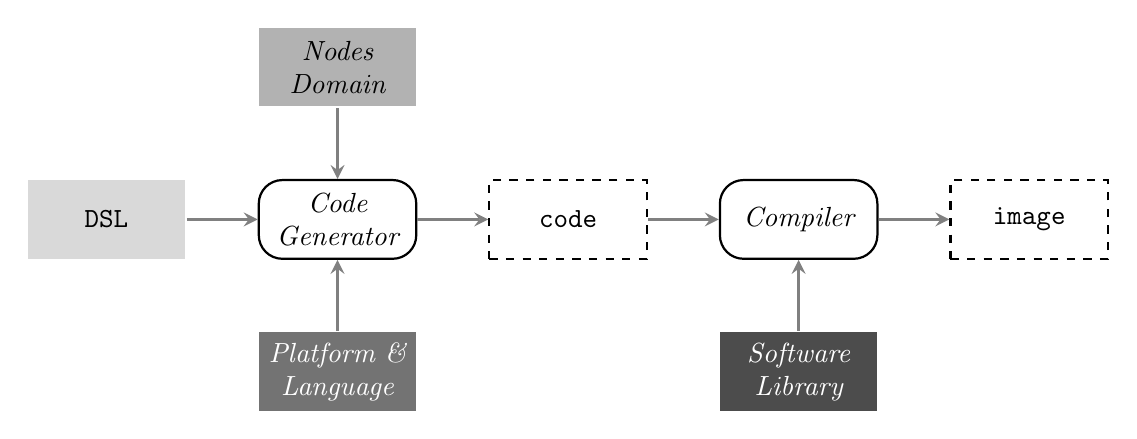
\begin{tikzpicture}[
  node distance=9mm,
  ,>=stealth,very thick,black!50,text=black,
  every new ->/.style={shorten >=1pt}
]
  \node (dsl)   [user]                                      {DSL};
  \node (cg)    [representation,right=of dsl,align=center]  {Code\\Generator};
  \node (code)  [generated,right=of cg]                     {code};
  \node (comp)  [representation,right=of code]              {Compiler};
  \node (image) [generated,right=of comp]                   {image};

  \node (nodes) [dom,above=of cg, align=center]             {Nodes\\Domain};
  \node (plat)  [platform,below=of cg,align=center]         {Platform \&\\Language};          
  \node (lib)   [native,below=of comp,align=center]         {Software\\Library};

  \draw [->] (dsl)   -> (cg);
  \draw [->] (nodes) -> (cg);
  \draw [->] (plat)  -> (cg);
  \draw [->] (cg)    -> (code);
  \draw [->] (code)  -> (comp);
  \draw [->] (lib)   -> (comp);
  \draw [->] (comp)  -> (image);

\end{tikzpicture}
}

\caption{The high level design of \NAME, showing the resources, processes and
artifacts. A grayscale background represents the level of platform dependency,
with darker shades indicating a higher dependency. Both the source code and the
installable image are artifacts.}

\label{fig:design}
\end{figure*}

\section{Design}
\label{design}

The previous sections identified loops, common data and the network as three
important code-level problems. These problems are inherent to ID algorithms.
But at the same time they conflict with the target environment, the IoT\@.
\NAME provides a framework to efficiently implement an IDS for the IoT and
offers a solution for the identified problems. It consists of a 1) DSL, 2)
source code generator and 3) software library. Figure \ref{fig:design}
visualizes the overall design.

% figure design is moved up to end up on this page

The DSL enables researchers to formally describe ID algorithms, without
focusing on any specific language or platform. A code generator can avoid the
identified problems concerning loops, common data and network access, as the
formal description provides the underlying intent, not the technical
implementation. It can also target different languages and platforms, while
reusing a software library that provides services including parsing, network
access wrapping,\dots

Using a DSL and code generator defines a development strategy. This has
implications, both on what is possible and how it can be achieved. We will
first position \NAME and motivate its design with respect to these trade offs.
Second, we will look at the principal design components of the DSL. Third, we
discuss the structure of the code generator and introduce its software library,
that offers a way to deal with for example the network access issue.

\subsection{\NAME as a Development Strategy}
\label{positioning}

The introduction of a code generator in the development process changes the
traditional way of working. Most importantly because the actual source code is
no longer the driving force that can be controlled by developers. It is
literally an intermediate representation between code generator and compiler.

A code generator constructs this representation using three components, as
shown in figure \ref{fig:design}: 1) the description of the algorithm in the
DSL, 2) information about the domain, in this case the Nodes domain and 3)
information about the platform and target language. At the level of the
compiler, a software library is introduced to offload specialized
implementations and allow custom extensions.

The applied grayscale indicates the components' platform dependency: the DSL is
platform and language independent and deals with subsystems, such as the
network, in an abstract way. The Nodes domain implements some of these
abstracted subsystems, but still in a platform and language independent way.
Platform and language descriptions convert the abstract constructions in
actually supported code. The software library is standard native code,
targeting the platform and language. Finally, the code and image are artifacts
of the automated generation and compilation process. They aren't a product of
manual work and therefore aren't directly dependent on the platform.

This hierarchy is important from a development effort point of view. The level
of dependency on the targeted platform dictates the level of effort to
implement changes to that platform. For example: to generate a different
language will require a complete rewrite of the software library and a partial
rewrite of the language description of the generator. Although this is a
reusable, one-time effort, it is important in relation to the scalability of
the framework itself.

\subsection{\NAME as a Domain Specific Language}
\label{dsl-design}

It's important to remember that a DSL is merely a \emph{thin veneer over a
(semantic) model} \cite{fowler2010domain}. Its sole purpose should be
populating the model. \NAME's DSL and model focus on avoiding constructions
that result in problems concerning loops, common data and the use of the
network. To do this, \NAME uses an event-based approach to defining
functionality.

Besides avoiding these problems, \NAME's DSL also provides a higher level of
abstraction with respect to memory management and data access.

This section therefore discusses \NAME's approach to 1) loops, 2) nodes domain,
3) unified messaging, 4) language support and illustrates these with a complete
example.

\subsubsection{Loops}

Loops are a major contributor to the problem of algorithm fusibility. Loops in
program code are technical constructs and in fact often hide the intended
functionality.

The example of parsing network messages illustrates this. Each algorithm deals
with parsing in the same way: loop over the bytes in the payload and look for a
pattern that identifies what the algorithm is looking for. This is in fact a
technical implementation choice. The underlying functional intent is to react
when such a pattern is present in a message. The loop has \emph{activated} this
functionality, but the real goal is to \emph{passively} react on an event, not
\emph{actively} look for it. Event handling therefore can transform
constructions with loops to their functional meaning, allowing identification
and fusion of common functionality.

The same goes for actively polling some variable until it reaches a certain
threshold. When transformed to a reaction to an event, it eliminates the need
for a technical loop-construction.

\subsubsection{The Nodes Domain}

Most, if not all, ID algorithms deal with information about other devices in
the network. To share this information \NAME provides a unified \ttt{nodes}
concept as part of its DSL and exposes it as an object to the implementer.

Algorithms can extend nodes with their own properties. This way, only one
instance for every known device will be present in memory. Finally, nodes can
define a scope for a function to execute in. This way, nodes offer a way to
i.e.\ iterate all known devices, again without the need for an explicit loop.

\subsubsection{Unified Messaging}
\label{dsl-unified-msg}

Access to the network, scattered around an algorithm, causes the wireless radio
to be more active than needed. Delaying the sending of messages and grouping
them, can lower this overhead.

Sending and receiving of network messages is tightly integrated with the
previously mentioned concepts of event handling and the Nodes domain. An
underlying software library can handle all interaction with the network,
triggering functions by means of events when parsing new messages and exposing
an API to send messages through the Nodes domain. This approach gives the
framework complete control over communication and for example allows for
optimized marshaling and grouping of messages.

\subsubsection{Language Support}
\label{language-support}

Using a platform independent language offers the possibility to relieve the
implementer of explicit memory management and low-level data structures. From a
language perspective, \NAME offers several programming constructs, typically
found in modern programming languages with higher levels of abstraction:
optional typing, object orientation, pattern matching, aspect orientation.

\subsubsection{An Example}

Listing \ref{lst:watchdog} illustrates some of the features mentioned above,
using a small but representative example of an algorithm: a watchdog
\cite{mishra2004intrusion}. Like a heartbeat, nodes can broadcast a message at
a regular interval, allowing other nodes to monitor its availability. Missing
heartbeats could indicate problems, such as physical capture of a device.

\lstinputlisting[
  language=foo-lang,
  float,
  basicstyle=\footnotesize\ttfamily\color{black},
  label=lst:watchdog,
  caption=Watchdog in \NAME
]{src/watchdog.foo}

\subsection{\NAME as a Code Generator}
\label{code-generator-design}

To convert the DSL-based ID algorithms into production-ready code, \NAME
applies code generation techniques. Although different approaches are
applicable, like template-based text expansion, XSLT transformations or CodeDom
\cite{dollard2004code}, we believe that the required transformations demand a
richer model.

A semantic model \cite{fowler2010domain}, tied closely to the DSL itself, can
fulfill this role. Semantic transformations evolve the model into a more
syntax-oriented model, comparable to the idea of CodeDom. From there on,
syntactic transformations can further evolve the model into source code. Figure
\ref{fig:code-generation} shows the process that \NAME implements.

\begin{figure}[ht]
  \centering
  \scalebox{.85}{
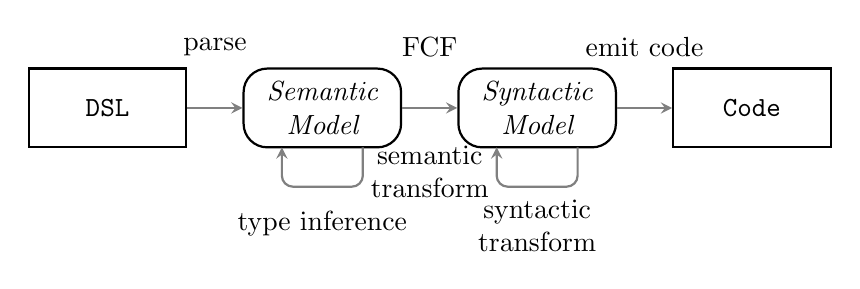
\begin{tikzpicture}[
  node distance=7mm,
  ,>=stealth,thick,black!50,text=black,
  every new ->/.style={shorten >=1pt}
]
  \node (dsl)  [resource]                                 {DSL};
  \node (sm)   [representation,right=of dsl,align=center] {Semantic\\Model};
  \node (cm)   [representation,right=of sm,align=center]  {Syntactic\\Model};
  \node (code) [resource,right=of cm]        {Code};


  \draw [->] (dsl) -> (sm)   node [midway,above=15pt]              {parse};
  \draw [->] (sm)  -> (cm)   node [midway,below=10pt,align=center] {semantic\\transform}
                             node [midway,above=15pt,align=center] {FCF};
  \draw [->] (cm)  -> (code) node [midway,above=15pt]              {emit code};

  \draw [rounded corners,->]
        ($ (sm.east) - (5mm,5mm) $)
        -- ++(0,-.5)
        -| ($ (sm.west) + (5mm,-5mm) $)
           node [near start, below=5pt] {type inference};

  \draw [rounded corners,->]
        ($ (cm.east) - (5mm,5mm) $)
        -- ++(0,-.5)
        -| ($ (cm.west) + (5mm,-5mm) $)
           node [near start, below=1pt,align=center] {syntactic\\transform};

\end{tikzpicture}
}
\caption{\NAME's code generation process}
\label{fig:code-generation}
\end{figure}

\subsubsection{Semantic Model}

The semantic model is the core of the solution. It offers a way to describe ID
algorithms in a way that allows semantic reinterpretation through functional
code fusion. This way, reorganizing the functionality of different algorithms
allows for more optimal execution and memory usage. Hence the name \NAME of the
framework: intrusion detection functionality organization optimization.

\begin{figure}[ht]
  \centering
  \scalebox{.85}{
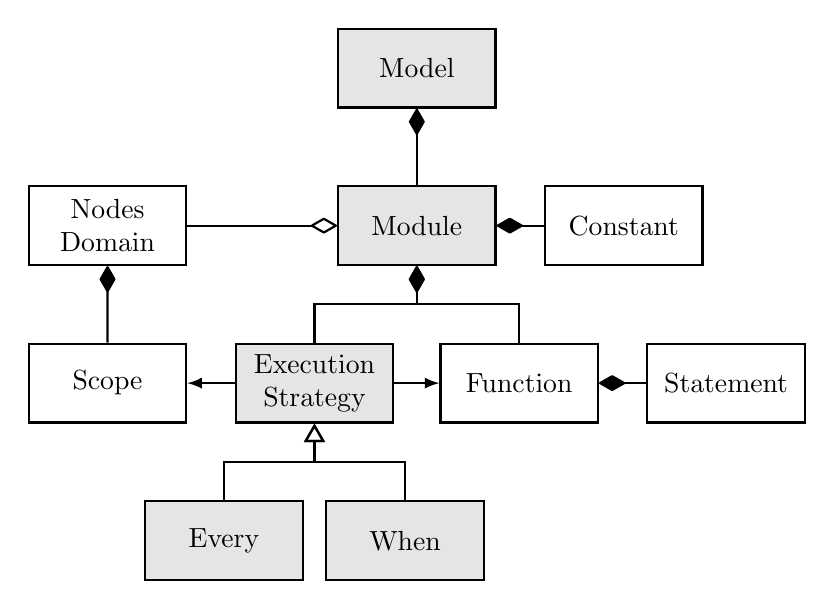
\begin{tikzpicture}[
  edge from parent fork down,
  sibling distance=5mm, level distance=20mm, node distance=6mm
  ]
  \node (model) [class,fill=black!10!white] {Model}
      child {node (module) [class,fill=black!10!white] {Module} edge from parent [composite]
        child {node (strategy) [class,align=center,xshift=-10.5mm,fill=black!10!white] {Execution\\Strategy} edge from parent [composite]
          child {node(every) [class,xshift=-9mm,fill=black!10!white] {Every} edge from parent [subclass]}
          child {node (when) [class,xshift=9mm,fill=black!10!white] {When} edge from parent [subclass]}
        }
        child {node (function) [class,xshift=10.5mm] {Function} edge from parent [composite]}
      };
  \node (constant)  [class,right=of module]   {Constant};
  \node (scope)     [class,left=of strategy]  {Scope};
  \node (statement) [class,right=of function] {Statement};
  \node (nodes)     [class,left=of module,xshift=-13mm]    {Nodes\\Domain};
  
  \draw [aggregate]  (module)   -- (nodes);
  \draw [composite]  (module)   -- (constant);
  \draw [dependency] (strategy) -- (scope);
  \draw [composite]  (function) -- (statement);
  
  \draw [composite]  (nodes)    -- (scope);
  \draw [dependency] (strategy) -- (function);
\end{tikzpicture}
}

\caption{Partial Semantic Model for \NAME. Shaded classes indicate the
\emph{event/scheduling} construction around functions to allow interpretation
of the intended functionality.}

\label{fig:meta-model}
\end{figure}

Figure \ref{fig:meta-model} shows the central part of the semantic model as
implemented for \NAME. The concept driving this model is the structure starting
at the \emph{Model} up to the \emph{Execution Strategy}. This structure
encompasses the \emph{Function}s and underlying \emph{Statement}s and allows
for interpretation and fusion of the algorithms.

\subsubsection{Functional Code Fusion (FCF)}

Thanks to the functional description of events and the effects triggered by
them, the code generator is able to identify the same actions across different
algorithms. This way it is possible to extract the parsing of incoming messages
and group actions on the same sets of data or scheduled function executions.

FCF typically looks for patterns in the semantic model and performs model
transformations to change these patterns to a more optimized organization. It
first performs semantic transformations on the semantic model itself. A second
phase transforms the semantic model into a syntactic model, encoding the
semantics into technical syntax constructs.

One example of a semantic transformation is type inference, which supports the
platform independence of the framework.

\subsubsection{Syntactic Model}

The syntactic model is like an abstract syntax tree (AST) for a virtual,
expressive language. It contains constructs and ideas found in different
languages and programming paradigms. No single existing programming language
supports all features as is. Syntactic transformations therefore translate the
unsupported constructs into comparable constructs supported by the targeted
platform and language.

Depending on the target platform, some constructions aren't transformed into
actually corresponding code. In selected cases, the generator uses a software
library. For example when it needs to parse incoming messages or schedule
tasks. During the generation process, it looks for patterns that indicate any
of these actions and transforms them into calls to the \NAME software library.

\subsection{\NAME as a Software Library}
\label{software-lib-design}

A software library allows offloading of common implementation aspects, thus
avoiding small discrepancies in code and suboptimal use of shared resources.
Section \ref{dsl-unified-msg} illustrated this approach with a case for unified
messaging: parsing of incoming messages and grouping of outgoing messages.

Other common functionality isn't generated as is either. The execution of
functions based on a schedule or the implementation of higher level conceptual
functions, such as \ttt{now} and \ttt{sha1}, are calls into the standard
software library.

Optimization of such algorithms is not within the scope of \NAME. This gives
freedom of choice to the users of the framework to select appropriate
implementations for this standard functionality.

\subsection{\NAME as a Framework}

\NAME reduces inefficiencies in network access, execution and memory usage,
that occur due to a selection of ID algorithms. To achieve this, it avoids
constructions that are hard to identify and reorganize, such as loops and
common data. A DSL, focussing on event-handling, enforces these restrictions
and enables formally describing ID algorithms.

The DSL is platform and language independent. This allows the source code
generator to target different configurations without any change to the formal
descriptions of the algorithms.

A supporting software library allows separation of standard functionality that
is out of scope for the generator. Optimization of the implementation of this
library for the specific platform and target language is possible.

% table goes here, because a spanning table is placed on the next page, relative
% to where it's defined.
\begin{table*}[b]
  \centering
  \begin{tabular}{llrrrrrrr}
\toprule
              &            & base  & \multicolumn{2}{c}{watchdog} & \multicolumn{2}{c}{reputation} & \multicolumn{2}{c}{both} \\
\midrule
\multirow{2}{*}{\pbox{\textwidth}{total packets sent\\in a window of 90s}}
              & manual     &    20 &    51 & +155\% &    32 &  +60\% &    63 & +215\%\\
              & generated  &    20 &    49 & +145\% &    32 &  +60\% &    55 & +175\%\\
\cmidrule{2-9}
              & difference &     0 &    -2 &   -4\% &     0 &   0\% &    -8 &   -13\%\\
\midrule
\multirow{2}{*}{\pbox{\textwidth}{total bytes sent\\in a window of 90s}}
              & manual     &   476 &  1933 & +306\% &   860 &  +81\% &  2317 & +387\%\\
              & generated  &   476 &  1897 & +299\% &   884 &  +86\% &  2161 & +354\%\\
\cmidrule{2-9}
              & difference &     0 &   -36 &   -2\% &    24 &   +3\% &  -156 &   -7\%\\
\midrule
\multirow{2}{*}{\pbox{\textwidth}{event loop\\average duration ($\mu$s)}}
              & manual     &    48 &    94 &  +96\% &    88 &  +83\% &   149 & +210\%\\
              & generated  &    48 &   121 & +152\% &   121 & +152\% &   138 & +188\%\\
\cmidrule{2-9}
              & difference &     0 &    27 &  +29\% &    33 &  +38\% &   -11 &   -7\%\\
\midrule
image
size (bytes)  & manual     & 10466 & 15530 &  +48\% & 13306 &  +27\% & 18334 &  +75\%\\
              & generated  & 10466 & 18352 &  +75\% & 16376 &  +56\% & 20998 & +101\%\\
\cmidrule{2-9}
              & difference &     0 &  2822 &  +18\% &  3070 &  +23\% &  2664 &  +15\%\\
\bottomrule
  \end{tabular}
  \caption{Results and Side-by-Side Comparison.}
  \label{tbl:results}
\end{table*}

\section{Implementation and Evaluation}
\label{evaluation}

In this section we present a prototype implementation and evaluate its
performance. We first present the implementation consisting of the hardware
platform, network and software stack. We first take an analytical approach and
look at the handling of common data and the size of the source code. Next, we
use the implementation to quantify its merits using a side-by-side comparison
of generated code versus a manual implementation. We consider experimental
results regarding usage of the network, execution time of the event-loop and
the image size.

\subsection{Implementation}

To evaluate the prototype we used a system based on the Atmel ATMEGA1284p
micro-controller and the Digi XBee S2 ZigBee module. A basic software library
wraps the technical calls to the hardware components in more easy to use
functions.

Relying on basic hardware and software allows us to validate that the generator
is capable of generating code even for the most basic environment. It shows
that the requirements of the generator towards the platform are minimal, don't
rely on advanced frameworks or operating systems and therefore are applicable
in any environment, targeting any platform.

For the evaluation we constructed a small meshed network. In this network, not
all devices have direct access to one another, requiring routing through shared
neighboring devices.

We started from a basic application that measures light intensity. The
application was an includable piece of code, which allowed integration in a
manual implementation and simple merging when generation. On top of this
baseline we added two intrusion detection related algorithms: a
watchdog \cite{mishra2004intrusion}, that allows nodes to validate each other's
presence, and a reputation-based algorithm \cite{ganeriwal2008reputation}, that
checks if a parent node is cooperative and actually forwards messages further
upstream.

\subsection{Analytical Results}

Looking at the generated source code is a straightforward way to validate the
framework. A simple metric is comparing the amount of code versus the size of
the formal description of ID algorithms. This can be an indication of the
development effort and complexity. In this experiment, implementing both
algorithms manually results in 637 lines of C code. The corresponding \NAME
implementation results in 156 lines of DSL code. This is largely thanks to the
higher level coding constructs, as introduced in section \ref{language-support}
dealing with \NAME's language support.

Next we look at data structures. Sharing data eliminates redundant information,
such as a network address, from the scope of each individual algorithm.
Analysis of the source code with both algorithms implemented, shows that this
reduces the memory footprint for one node entry by 2 bytes, from 27 bytes to 25
bytes. In our implementation we used the ZigBee network address, which indeed
consists of 16 bits. This results in a reduction of 7.4\%. Using ZigBee's 64
bits unique addresses, this reduction can easily become 20.5\%.

\subsection{Experimental Results}

Besides this analysis we also instrumented the code and evaluated four
criteria: the network usage in number of packets and bytes, the time required
to perform once cycle of the event loop and the image size of the resulting
compiled code. To do this, we collected these metrics for four situations:
without ID algorithms, with a watchdog, with reputation-tracking and with both
algorithms implemented.

The manual implementation realized both algorithms as standalone modules and
sequentially called them from the base-application's event loop. Given the
\NAME descriptions of the algorithms, the code generator generated all four
cases.

Table \ref{tbl:results} shows the collected data for the manual and the
generated implementation, as well as a comparison in absolute values and
relative.

These results show that adding algorithms manually to the base-application has
a cumulative effect. The impact of both algorithms is simply the sum of the
impact of each algorithm by itself. The execution time of one cycle of the
event loop with both algorithms enabled is even higher than simply the sum.

In case of the generated implementation, this effect is no longer observed:
individual algorithms do have a larger impact by themselves, but the
combination of both algorithms is less than the sum of both.

Most remarkable is the effect on the time of one event loop cycle: both
algorithms by itself add 152\%. Adding a second algorithm only augments the
impact to 188\%. We see the effect of the generic handling of common
functionality, like message parsing and event scheduling. It comes with an
overhead for a single algorithm, but pays for itself when adding more
algorithms.

Table \ref{tbl:results} also compares the two situations by subtracting the
manual case from the generated case, showing the impact of the code generation.
A relative value for this difference, to the manual case, is also included.
Four observations allow us to evaluate the overall performance of \NAME's
approach.

The first observation deals with the base case: both the manual and the
generated implementations perform exactly the same. There is no fundamental
structural difference in the overall architecture of the code.

Secondly, when turning to the goal to reduce the network usage, we see that
both the number of packets as well as the amount of bytes sent have dropped by
13\% and 7\%.

Thirdly, focusing on the execution time, both algorithms by themselves add an
equal amount of time to the processing of a single event loop cycle. But when
combined, the event loop is about 7\% faster compared to the manual case.

Finally, we see that the software library that comes with the generated code
adds to the size of the resulting image. But the cost is close to constant and
is lower for both algorithms together. With roughly 3KB of additional overhead,
or 15\% in this simple case, the impact is small. Taking into account the
available memory on the ATMega1284p, this is only 2.3\% of the available
resources.

\section{Related Work}
\label{related}

Section \ref{classification} introduced some ID algorithms
\cite{ganeriwal2008reputation,mishra2004intrusion,krontiris2009cooperative} and
presented a classification
\cite{mishra2004intrusion,ioannis2007towards,alrajeh2013intrusion} based on
their detection approach and interaction style.

This section focuses on related work in the field of domain specific languages
and code generation, both in relation to wireless networks of
resource-constrained devices. These two components are the core of the \NAME
framework and the solution it proposes. We also look at their application in
other disciplines and how this can relate to our context.

\subsection{Domain Specific Languages}

Within the scope of wireless networks of resource-constrained devices, we see
the introduction of DSLs \enquote{to shorten the development cycles
dramatically during deployments, to reduce the dependency on hardware and
software engineers, and to lead to a wider adoption outside the computer
science field} \cite{sadilek2008domain}.

TinyScript \cite{levis2004tinyscript} is an example of a language for wireless
sensor networks. It's a complete programing language that aims to ease the
description of algorithms in general. The Basic-like syntax does enable more
productive development. But this approach doesn't address the underlying
resource problems inherently connected to the context.

SEAL \cite{elsts2013seal} is a novel complete programming language that focuses
on novice programmers. It is a clear fit for \emph{sense-and-send} type of
applications. It does however share the idea of events to overcome the technical
nature of loops.

Shifting the scope to intrusion detection, we learn that DSLs are predominantly
used to describe patterns of events found in network
packets \cite{sekar1999high,roesch1999snort} in a concise way.

BMSL \cite{uppuluri2001experiences} is a DSL that allows the specification of
patterns and actions. Patterns can contain events extracted from log files,
system calls and network packets.

The STAT framework with its STATL language
\cite{eckmann2002statl,vigna2003designing} are not intrusion detection
specific, but through extensions they allow to model attack scenarios using
state machines. Our event-driven approach shares these same ideas.

Although not a real DSL, nesC \cite{gay2003nesc} is a general purpose language
that shares some typical concepts with \NAME, such as the high degree of
analysis during code generation to optimize execution. The biggest difference
is that \NAME starts from the intended functionality and can optimize certain
constructions that can't be interpreted from more technical source code.

\subsection{Code Generation}

Code generation, in combination with a DSL, can optimize a development process
by reducing the size of the code base or systematically improving the code
quality.

Embedded systems are a prime example of an environment where code needs to be
of a high quality. Focus on size and performance are a logical choice when
dealing with limited storage and processing power. Compilers implement
different techniques to address this at the lowest level
\cite{marwedel2002code}.

Optimizing for power efficiency however proves to be concurrent to size and
performance optimization, and requires different strategies. Data and memory
optimizations \cite{panda2001data} can result in improvements on a lower level.
But really preserving energy requires higher-level strategies, targeting
architecture, radio handling, efficient software,\dots \cite{naik2001software}.
Most of these are beyond the control of the compiler and require a higher level
of abstraction to address them.

DSLs offer a solution here, but other paradigms are possible. A mixed framework
consisting of a virtual machine (VM) and native code extension
\cite{sadilek2007energy}, combined with energy-aware compilation, seems a
promising approach. By offloading the optimization to a VM and only compiling
parts and not the whole, the solution allows updating at a granular scale, thus
reducing the update cost, while maintaining flexibility and lowering the
development effort. In this terminology, \NAME focuses on the reduction of the
development effort and update cost, and maximizes flexibility.

Applying code generation to ID, often focusses on the generation of native code
to avoid the interpretation of descriptions of patterns to look for. I2S
\cite{charitakis2003code} is an example that generates code for SNORT
\cite{roesch1999snort} rules. To optimize this highly efficient code, it often
targets a specific platform.

\section{Conclusion and Future Work}
\label{conclusion}

Adequate intrusion detection for IoT devices requires multiple algorithms to
operate at the same time. Frequent reselection, e.g. due to changing
requirements or security threats, requires a flexible way to incorporate the
different algorithms.

Adding multiple intrusion detection algorithms to wireless resource-constrained
devices requires fusion of algorithms on a functional level. This can reduce
execution inefficiencies as well as redundant memory usage and network access.

\NAME is a framework consisting of a DSL, a source code generator and software
library. Using the DSL, intrusion detection algorithms can be formally
described. The code generator applies functional code fusion to interpret the
intent of algorithms and merges common functionality and shared data. The
software library hosts common functionality, such as network message parsing
and event scheduling.

Initial experiments confirm the theoretical positive impact on resource usage:
grouping of messages lowers the number of packets by 13\%, while the total
number of bytes sent over the network is reduced by 7\%. The execution time is
improved by 7\% and memory usage can be reduced by even 20\%.

The platform independent DSL enables generation of source code targeting
different platforms and languages, which allows high degrees of reuse with
heterogenous devices.

As a next step, we will implement more ID algorithms using \NAME and continue
the experiments on a larger scale. This way we will also be able to verify the
initially observed inclination in the evolution of the image size with growing
numbers of algorithms.

Future research will focus on the integration of applications with a generated
IDS. We see opportunities for applications who detect intrusions, to actively
and dynamically respond and avoid malicious payloads.

A continued effort is targeting the reduction of platform-dependent parts in
the implementation. This way it is possible to add more platforms and languages
with less effort.

In the longer run, we want to investigate the possibility to extend the
functional code fusion paradigm to other domains beyond intrusion detection.

\section{Acknowledgements}

This research is partially funded by the Research Fund KU Leuven and partially
by the EU FP7 project NESSoS\@.

\bibliographystyle{IEEEtran}
\bibliography{literature/referenties}

\end{document}
